\documentclass[10pt,a4paper,landscape]{report}
\usepackage[dutch]{babel}
\usepackage{amsmath}
\usepackage{amsfonts}
\usepackage{amssymb}
\usepackage{graphicx}
\usepackage{tikz}
\usepackage{environ}
\makeatletter
\newsavebox{\measure@tikzpicture}
\NewEnviron{scaletikzpicturetowidth}[1]{%
  \def\tikz@width{#1}%
  \def\tikzscale{1}\begin{lrbox}{\measure@tikzpicture}%
  \BODY
  \end{lrbox}%
  \pgfmathparse{#1/\wd\measure@tikzpicture}%
  \edef\tikzscale{\pgfmathresult}%
  \BODY
}
\makeatother
\usepackage[left=2cm,right=2cm,top=3cm,bottom=3cm]{geometry}
\author{Aranka Steyaert}
\begin{document}
\begin{scaletikzpicturetowidth}{\linewidth}
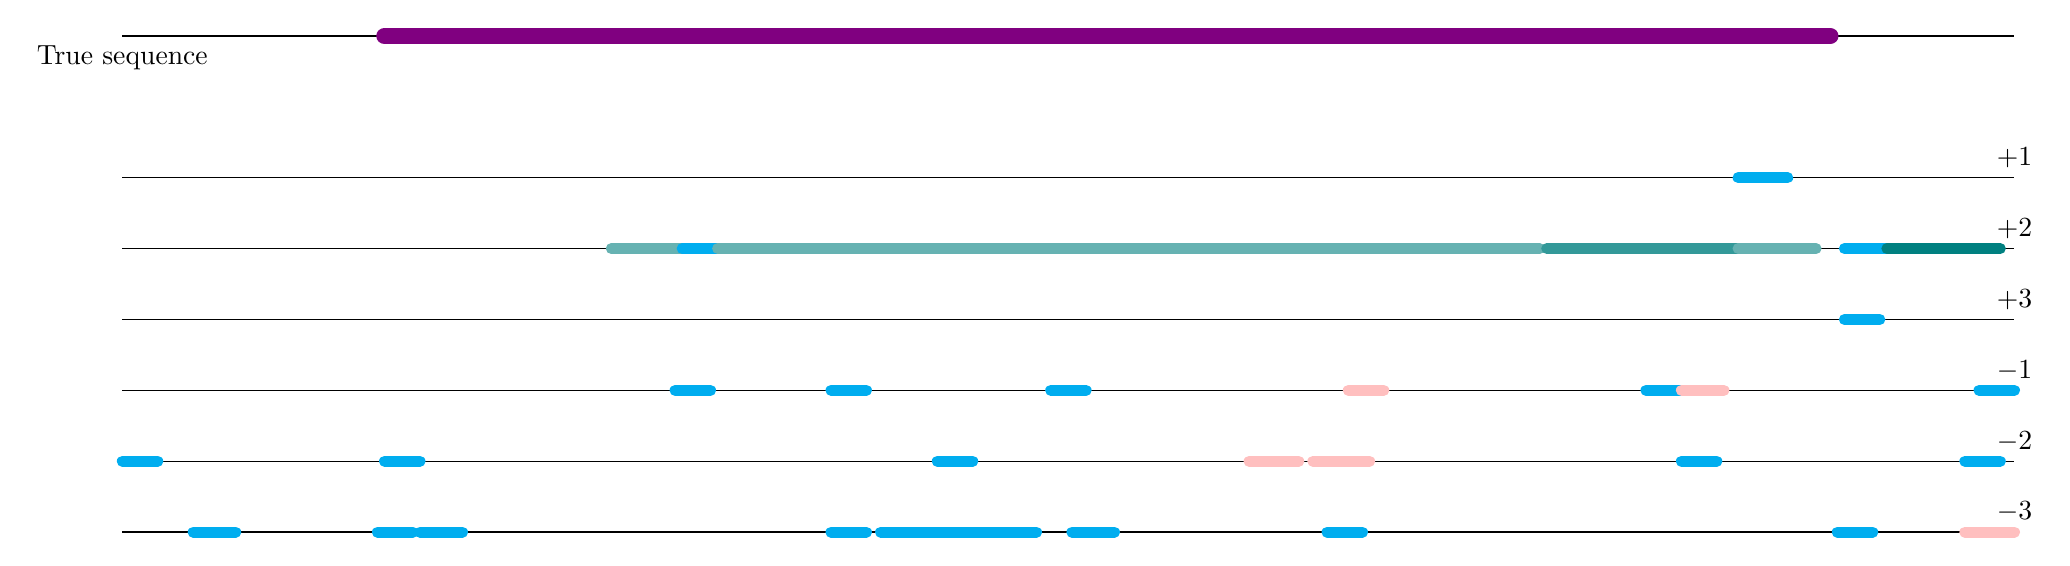
\begin{tikzpicture}
[scale=0.9,
protein/.style={violet, line width = 6pt, line cap = round},
root/.style={cyan, line width = 4pt, line cap = round},
genus/.style={teal!60, line width = 4pt, line cap = round},
species/.style={teal, line width = 4pt, line cap = round},
species group/.style={teal!80, line width = 4pt, line cap = round},
wrong/.style={pink, line width = 4pt, line cap = round},
superkingdom/.style={teal!10, line width = 4pt, line cap = round}]
\draw node[anchor=north] {True sequence} (0,0) -- (26.7,0) ;
\draw (0,-2) -- (26.7,-2) node[anchor=south] {$+1$};
\draw (0,-3) -- (26.7,-3) node[anchor=south] {$+2$};
\draw (0,-4) -- (26.7,-4) node[anchor=south] {$+3$};
\draw (0,-5) -- (26.7,-5) node[anchor=south] {$-1$};
\draw (0,-6) -- (26.7,-6) node[anchor=south] {$-2$};
\draw (0,-7) -- (26.7,-7) node[anchor=south] {$-3$};
\draw[protein] (3.7,0) -- (24.1,0);
\draw[root] (22.8,-2) -- (23.5,-2);
\draw[genus] (6.9,-3)--(7.9,-3);
\draw[root] (7.9,-3)--(8.4,-3);
\draw[genus] (8.4,-3)--(11.7,-3);
\draw[genus] (11.7,-3)--(14.5,-3);
\draw[genus] (14.5,-3)--(17.3,-3);
\draw[genus] (17.3,-3)--(20,-3);
\draw[species group] (20.1,-3)--(22.8,-3);
\draw[genus] (22.8,-3)--(23.9,-3);
\draw[root] (24.3,-3)--(24.9,-3);
\draw[species] (24.9,-3)--(26.5,-3);
\draw[root] (24.3,-4)--(24.8,-4);
\draw[root] (7.8,-5)--(8.3,-5);
\draw[root] (10,-5)--(10.5,-5);
\draw[root] (13.1,-5)--(13.6,-5);
\draw[wrong] (17.3,-5)--(17.8,-5);
\draw[root] (21.5,-5)--(22,-5);
\draw[wrong] (22,-5)--(22.6,-5);
\draw[root] (26.2,-5)--(26.7,-5);
\draw[root] (0,-6)--(0.5,-6);
\draw[root] (3.7,-6)--(4.2,-6);
\draw[root] (11.5,-6)--(12,-6);
\draw[wrong] (15.9,-6)--(16.6,-6);
\draw[wrong] (16.8,-6)--(17.6,-6);
\draw[root] (22,-6)--(22.5,-6);
\draw[root] (26,-6)--(26.5,-6);
\draw[root] (1,-7)--(1.6,-7);
\draw[root] (3.6,-7)--(4.1,-7);
\draw[root] (4.2,-7)--(4.8,-7);
\draw[root] (10,-7)--(10.5,-7);
\draw[root] (10.7,-7)--(11.4,-7);
\draw[root] (11.4,-7)--(11.9,-7);
\draw[root] (11.9,-7)--(12.4,-7);
\draw[root] (12.4,-7)--(12.9,-7);
\draw[root] (13.4,-7)--(14,-7);
\draw[root] (17,-7)--(17.5,-7);
\draw[root] (24.2,-7)--(24.7,-7);
\draw[wrong] (26,-7)--(26.7,-7);
\end{tikzpicture}
\end{scaletikzpicturetowidth}

Het stuk dat buiten de proteine ligt, wordt in andere assemblies van Acinetobacter Baumannii wel ge\"identificeerd als een hypothetische prote\"ine van Acinetobacte baumannii (na BLASTp).

\begin{scaletikzpicturetowidth}{\linewidth}
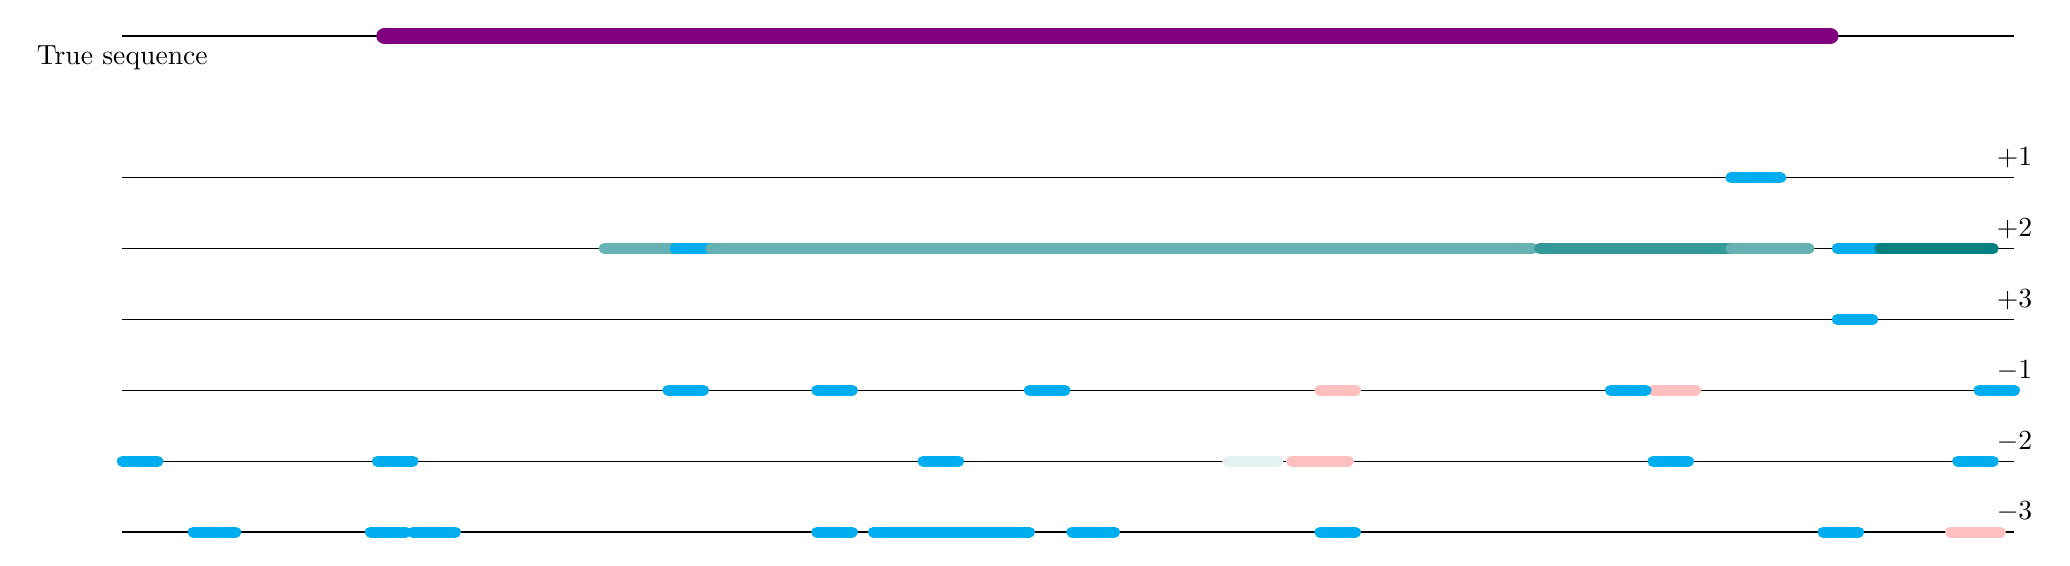
\begin{tikzpicture}
[scale=0.9,
root/.style={cyan, line width = 4pt, line cap = round},
genus/.style={teal!60, line width = 4pt, line cap = round},
species/.style={teal, line width = 4pt, line cap = round},
species group/.style={teal!80, line width = 4pt, line cap = round},
wrong/.style={pink, line width = 4pt, line cap = round},
superkingdom/.style={teal!10, line width = 4pt, line cap = round}]
\draw node[anchor=north] {True sequence} (0,0) -- (26.7,0) ;
\draw (0,-2) -- (26.7,-2) node[anchor=south] {$+1$};
\draw (0,-3) -- (26.7,-3) node[anchor=south] {$+2$};
\draw (0,-4) -- (26.7,-4) node[anchor=south] {$+3$};
\draw (0,-5) -- (26.7,-5) node[anchor=south] {$-1$};
\draw (0,-6) -- (26.7,-6) node[anchor=south] {$-2$};
\draw (0,-7) -- (26.7,-7) node[anchor=south] {$-3$};
\draw[violet, line width = 6pt, line cap = round] (3.7,0) -- (24.1,0);
\draw[root] (22.7,-2) -- (23.4,-2);
\draw[genus] (6.8,-3) -- (7.8,-3);
\draw[root] (7.8,-3) -- (8.3,-3);
\draw[genus] (8.3,-3) -- (11.600000000000001,-3);
\draw[genus] (11.6,-3) -- (14.399999999999999,-3);
\draw[genus] (14.4,-3) -- (17.2,-3);
\draw[genus] (17.2,-3) -- (19.9,-3);
\draw[species group] (20.0,-3) -- (22.7,-3);
\draw[genus] (22.7,-3) -- (23.8,-3);
\draw[root] (24.2,-3) -- (24.8,-3);
\draw[species] (24.8,-3) -- (26.400000000000002,-3);
\draw[root] (24.2,-4) -- (24.7,-4);
\draw[root] (26.2,-5) -- (26.7,-5);
\draw[wrong] (21.599999999999998,-5) -- (22.2,-5);
\draw[root] (21.0,-5) -- (21.5,-5);
\draw[wrong] (16.9,-5) -- (17.4,-5);
\draw[root] (12.799999999999999,-5) -- (13.299999999999999,-5);
\draw[root] (9.8,-5) -- (10.3,-5);
\draw[root] (7.699999999999999,-5) -- (8.2,-5);
\draw[root] (25.900000000000002,-6) -- (26.400000000000002,-6);
\draw[root] (21.6,-6) -- (22.1,-6);
\draw[wrong] (16.5,-6) -- (17.3,-6);
\draw[superkingdom] (15.600000000000001,-6) -- (16.3,-6);
\draw[root] (11.3,-6) -- (11.8,-6);
\draw[root] (3.6000000000000014,-6) -- (4.100000000000001,-6);
\draw[root] (0.0,-6) -- (0.5,-6);
\draw[wrong] (25.8,-7) -- (26.5,-7);
\draw[root] (24.0,-7) -- (24.5,-7);
\draw[root] (16.900000000000002,-7) -- (17.400000000000002,-7);
\draw[root] (13.400000000000002,-7) -- (14.000000000000002,-7);
\draw[root] (12.3,-7) -- (12.8,-7);
\draw[root] (11.8,-7) -- (12.3,-7);
\draw[root] (11.3,-7) -- (11.8,-7);
\draw[root] (10.600000000000001,-7) -- (11.3,-7);
\draw[root] (9.8,-7) -- (10.3,-7);
\draw[root] (4.100000000000003,-7) -- (4.700000000000003,-7);
\draw[root] (3.5,-7) -- (4.0,-7);
\draw[root] (1.0000000000000013,-7) -- (1.6000000000000014,-7);
\end{tikzpicture}
\end{scaletikzpicturetowidth}

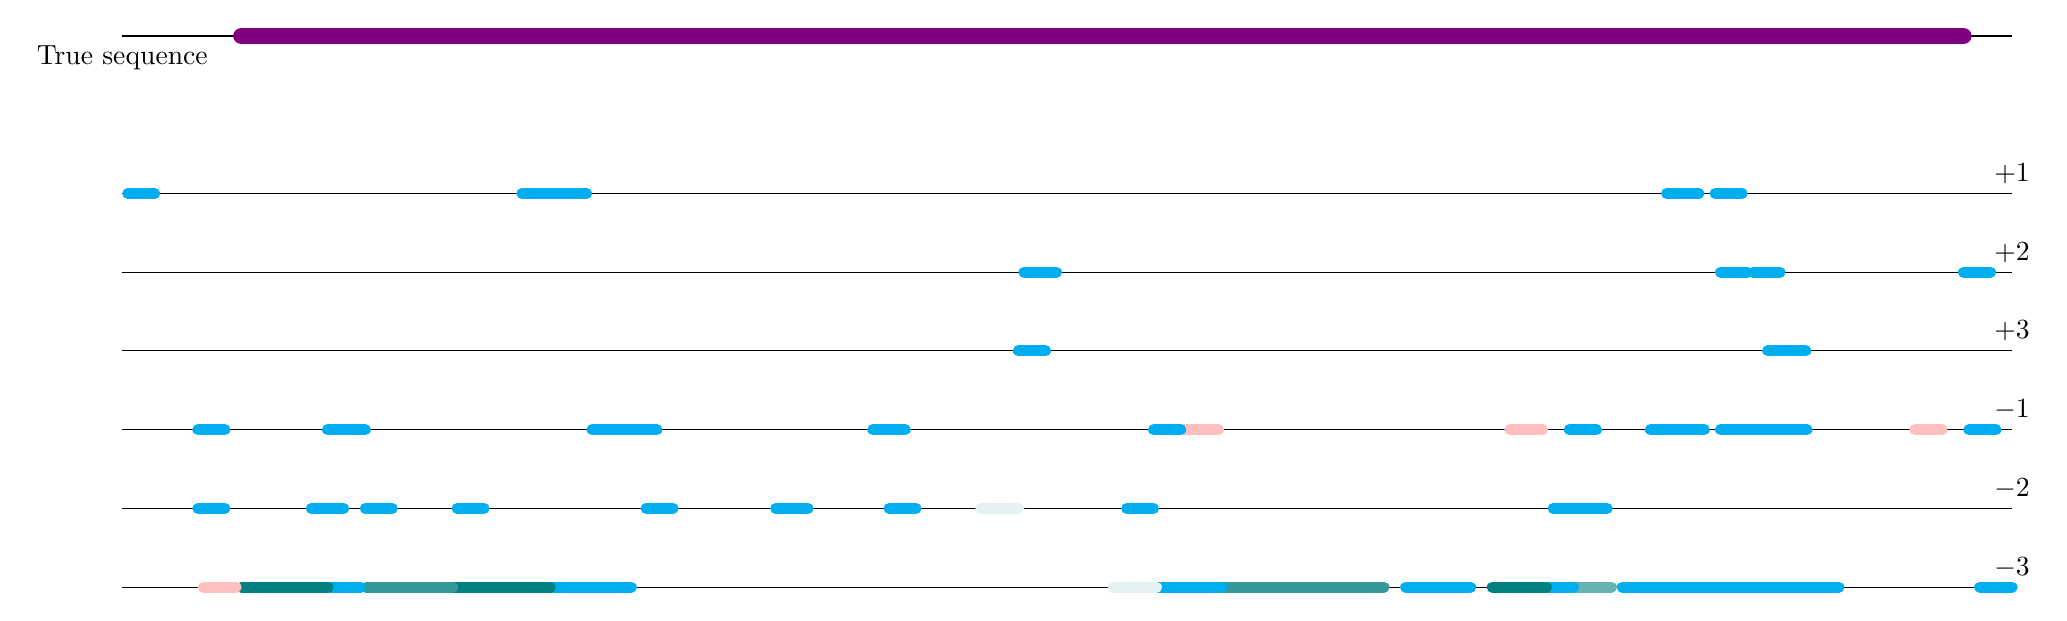
\begin{tikzpicture}
[protein/.style={violet, line width = 6pt, line cap = round},
root/.style={cyan, line width = 4pt, line cap = round},
genus/.style={teal!60, line width = 4pt, line cap = round},
species/.style={teal, line width = 4pt, line cap = round},
species group/.style={teal!80, line width = 4pt, line cap = round},
wrong/.style={pink, line width = 4pt, line cap = round},
superkingdom/.style={teal!10, line width = 4pt, line cap = round}]
\draw node[anchor=north] {True sequence} (0,0) -- (24,0) ;
\draw (0,-2) -- (24,-2) node[anchor=south] {$+1$};
\draw (0,-3) -- (24,-3) node[anchor=south] {$+2$};
\draw (0,-4) -- (24,-4) node[anchor=south] {$+3$};
\draw (0,-5) -- (24,-5) node[anchor=south] {$-1$};
\draw (0,-6) -- (24,-6) node[anchor=south] {$-2$};
\draw (0,-7) -- (24,-7) node[anchor=south] {$-3$};
\draw[root] (0.06857142857142857,-2) -- (0.4114285714285714,-2);
\draw[root] (5.074285714285715,-2) -- (5.554285714285715,-2);
\draw[root] (5.554285714285714,-2) -- (5.897142857142857,-2);
\draw[root] (19.611428571428572,-2) -- (20.022857142857145,-2);
\draw[root] (20.22857142857143,-2) -- (20.571428571428573,-2);
\draw[root] (11.451428571428572,-3) -- (11.862857142857143,-3);
\draw[root] (20.29714285714286,-3) -- (20.64,-3);
\draw[root] (20.708571428571428,-3) -- (21.05142857142857,-3);
\draw[root] (23.382857142857144,-3) -- (23.725714285714286,-3);
\draw[root] (11.379310344827585,-4) -- (11.724137931034482,-4);
\draw[root] (20.896551724137932,-4) -- (21.379310344827587,-4);
\draw[root] (23.451428571428572,-5) -- (23.794285714285714,-5);
\draw[wrong] (22.76571428571429,-5) -- (23.10857142857143,-5);
\draw[root] (21.051428571428573,-5) -- (21.394285714285715,-5);
\draw[root] (20.708571428571428,-5) -- (21.05142857142857,-5);
\draw[root] (20.297142857142855,-5) -- (20.708571428571428,-5);
\draw[root] (19.74857142857143,-5) -- (20.091428571428573,-5);
\draw[root] (19.405714285714286,-5) -- (19.748571428571427,-5);
\draw[root] (18.377142857142857,-5) -- (18.72,-5);
\draw[wrong] (17.622857142857143,-5) -- (18.034285714285716,-5);
\draw[wrong] (13.44,-5) -- (13.92,-5);
\draw[root] (13.097142857142856,-5) -- (13.44,-5);
\draw[root] (9.53142857142857,-5) -- (9.942857142857141,-5);
\draw[root] (6.3771428571428554,-5) -- (6.7885714285714265,-5);
\draw[root] (5.965714285714286,-5) -- (6.377142857142857,-5);
\draw[root] (2.6057142857142854,-5) -- (3.0857142857142854,-5);
\draw[root] (0.9599999999999996,-5) -- (1.3028571428571425,-5);
\draw[root] (18.514285714285716,-6) -- (18.857142857142858,-6);
\draw[root] (18.17142857142857,-6) -- (18.514285714285712,-6);
\draw[root] (12.754285714285713,-6) -- (13.097142857142856,-6);
\draw[superkingdom] (10.902857142857142,-6) -- (11.382857142857143,-6);
\draw[root] (9.737142857142857,-6) -- (10.08,-6);
\draw[root] (8.297142857142857,-6) -- (8.708571428571428,-6);
\draw[root] (6.65142857142857,-6) -- (6.994285714285713,-6);
\draw[root] (4.251428571428572,-6) -- (4.594285714285714,-6);
\draw[root] (3.085714285714284,-6) -- (3.428571428571427,-6);
\draw[root] (2.4,-6) -- (2.8114285714285714,-6);
\draw[root] (0.9599999999999996,-6) -- (1.3028571428571425,-6);
\draw[protein] (1.5128939828080235,0) -- (23.3810888252149,0);
\draw[root] (23.587392550143267,-7) -- (24.0,-7);
\draw[root] (20.492836676217767,-7) -- (21.799426934097422,-7);
\draw[root] (19.80515759312321,-7) -- (20.492836676217763,-7);
\draw[root] (19.46131805157593,-7) -- (19.80515759312321,-7);
\draw[root] (19.048710601719197,-7) -- (19.46131805157593,-7);
\draw[genus] (18.429799426934096,-7) -- (18.911174785100286,-7);
\draw[root] (18.085959885386817,-7) -- (18.429799426934096,-7);
\draw[species] (17.398280802292266,-7) -- (18.08595988538682,-7);
\draw[root] (16.297994269340975,-7) -- (17.12320916905444,-7);
\draw[species group] (14.578796561604586,-7) -- (16.022922636103154,-7);
\draw[species group] (13.959885386819483,-7) -- (14.578796561604584,-7);
\draw[root] (13.134670487106018,-7) -- (13.959885386819485,-7);
\draw[superkingdom] (12.584527220630372,-7) -- (13.134670487106018,-7);
\draw[root] (5.432664756446993,-7) -- (6.4641833810888265,-7);
\draw[species] (4.194842406876789,-7) -- (5.432664756446989,-7);
\draw[species group] (3.094555873925502,-7) -- (4.194842406876791,-7);
\draw[root] (2.6131805157593133,-7) -- (3.025787965616047,-7);
\draw[species] (1.5128939828080212,-7) -- (2.6131805157593107,-7);
\draw[wrong] (1.0315186246418326,-7) -- (1.4441260744985662,-7);
\end{tikzpicture}

\vspace{2cm}
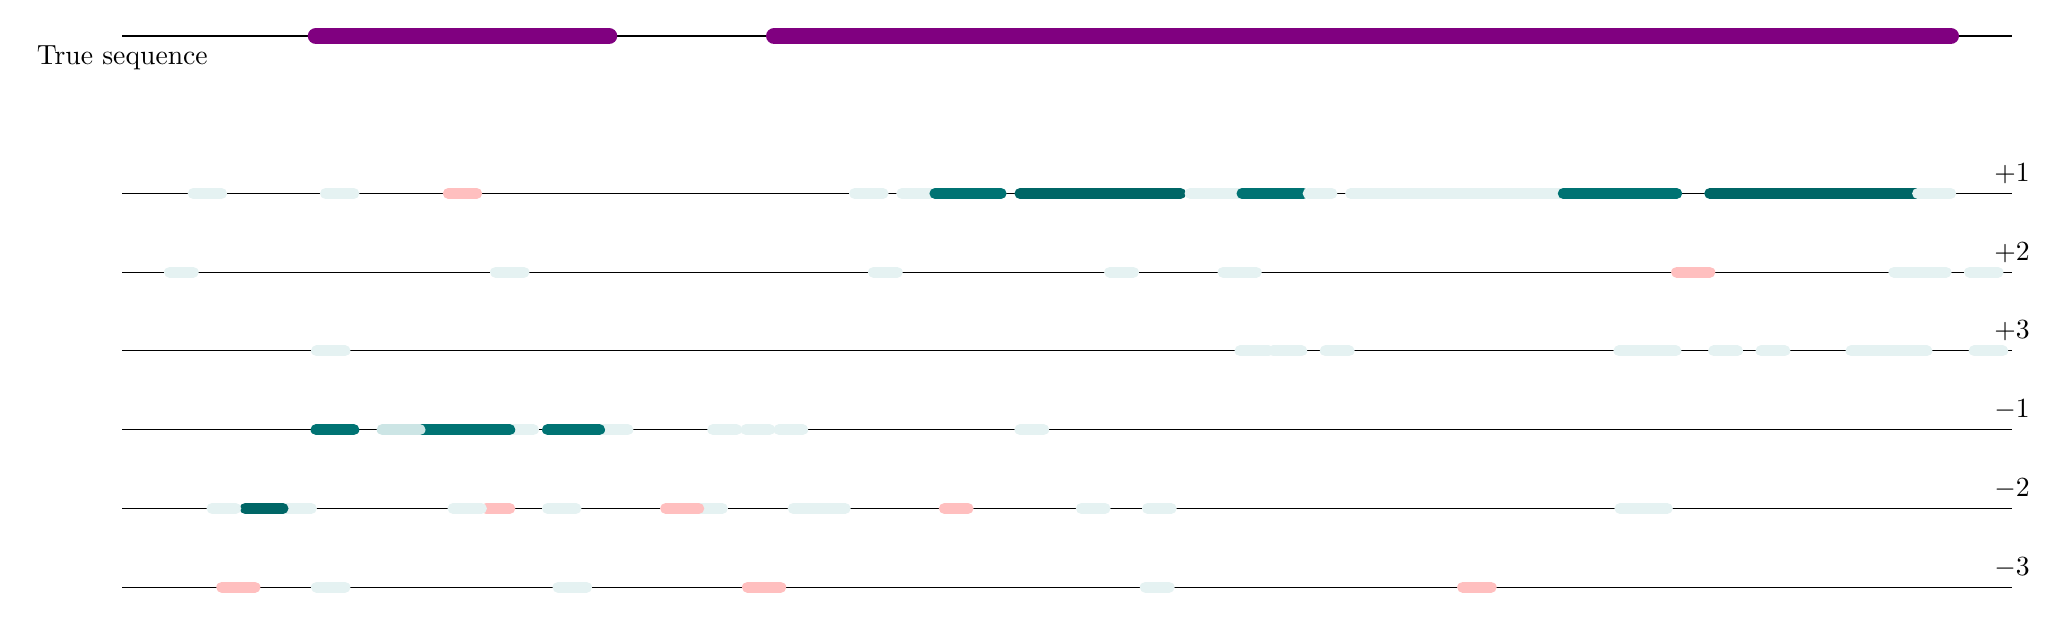
\begin{tikzpicture}
[protein/.style={violet, line width = 6pt, line cap = round},
root/.style={teal!10, line width = 4pt, line cap = round},
genus/.style={teal, line width = 4pt, line cap = round},
species/.style={teal!80!black, line width = 4pt, line cap = round},
species group/.style={teal!90!black, line width = 4pt, line cap = round},
wrong/.style={pink, line width = 4pt, line cap = round},
superkingdom/.style={teal!20, line width = 4pt, line cap = round}]
\draw node[anchor=north] {True sequence} (0,0) -- (24,0) ;
\draw (0,-2) -- (24,-2) node[anchor=south] {$+1$};
\draw (0,-3) -- (24,-3) node[anchor=south] {$+2$};
\draw (0,-4) -- (24,-4) node[anchor=south] {$+3$};
\draw (0,-5) -- (24,-5) node[anchor=south] {$-1$};
\draw (0,-6) -- (24,-6) node[anchor=south] {$-2$};
\draw (0,-7) -- (24,-7) node[anchor=south] {$-3$};
\draw[protein] (8.28,0) -- (23.22,0);
\draw[root] (0.8999999999999999,-2) -- (1.2599999999999998,-2);
\draw[root] (2.58,-2) -- (2.94,-2);
\draw[wrong] (4.14,-2) -- (4.5,-2);
\draw[root] (9.299999999999999,-2) -- (9.659999999999998,-2);
\draw[root] (9.9,-2) -- (10.26,-2);
\draw[species group] (10.32,-2) -- (11.16,-2);
\draw[species] (11.4,-2) -- (13.440000000000001,-2);
\draw[root] (13.559999999999999,-2) -- (14.219999999999999,-2);
\draw[species group] (14.219999999999999,-2) -- (14.999999999999998,-2);
\draw[root] (15.059999999999999,-2) -- (15.36,-2);
\draw[root] (15.6,-2) -- (17.34,-2);
\draw[root] (17.34,-2) -- (17.64,-2);
\draw[root] (17.64,-2) -- (18.3,-2);
\draw[species group] (18.3,-2) -- (19.740000000000002,-2);
\draw[species] (20.16,-2) -- (21.36,-2);
\draw[species] (21.36,-2) -- (22.8,-2);
\draw[root] (22.8,-2) -- (23.220000000000002,-2);
\draw[root] (0.6,-3) -- (0.8999999999999999,-3);
\draw[root] (4.74,-3) -- (5.1000000000000005,-3);
\draw[root] (9.54,-3) -- (9.84,-3);
\draw[root] (12.54,-3) -- (12.84,-3);
\draw[root] (13.979999999999999,-3) -- (14.399999999999999,-3);
\draw[wrong] (19.74,-3) -- (20.16,-3);
\draw[root] (22.5,-3) -- (22.86,-3);
\draw[root] (22.86,-3) -- (23.16,-3);
\draw[root] (23.46,-3) -- (23.82,-3);
\draw[root] (2.4661654135338344,-4) -- (2.827067669172932,-4);
\draw[root] (14.19548872180451,-4) -- (14.556390977443609,-4);
\draw[root] (14.616541353383457,-4) -- (14.977443609022554,-4);
\draw[root] (15.278195488721803,-4) -- (15.578947368421051,-4);
\draw[root] (19.00751879699248,-4) -- (19.308270676691727,-4);
\draw[root] (19.308270676691727,-4) -- (19.729323308270676,-4);
\draw[root] (20.210526315789473,-4) -- (20.51127819548872,-4);
\draw[root] (20.81203007518797,-4) -- (21.112781954887218,-4);
\draw[root] (21.954887218045112,-4) -- (22.31578947368421,-4);
\draw[root] (22.31578947368421,-4) -- (22.616541353383457,-4);
\draw[root] (22.616541353383457,-4) -- (22.917293233082706,-4);
\draw[root] (23.518796992481203,-4) -- (23.8796992481203,-4);
\draw[protein] (2.46,0) -- (6.18,0);
\draw[root] (11.4,-5) -- (11.700000000000001,-5);
\draw[root] (8.34,-5) -- (8.64,-5);
\draw[root] (7.920000000000001,-5) -- (8.22,-5);
\draw[root] (7.500000000000001,-5) -- (7.800000000000001,-5);
\draw[root] (6.060000000000001,-5) -- (6.420000000000002,-5);
\draw[species group] (5.400000000000002,-5) -- (6.060000000000002,-5);
\draw[root] (4.920000000000003,-5) -- (5.220000000000002,-5);
\draw[species group] (4.320000000000002,-5) -- (4.920000000000002,-5);
\draw[species group] (3.7800000000000002,-5) -- (4.32,-5);
\draw[superkingdom] (3.300000000000001,-5) -- (3.780000000000001,-5);
\draw[species group] (2.4600000000000013,-5) -- (2.9400000000000013,-5);
\draw[root] (19.32,-6) -- (19.62,-6);
\draw[root] (19.02,-6) -- (19.32,-6);
\draw[root] (13.02,-6) -- (13.32,-6);
\draw[root] (12.18,-6) -- (12.48,-6);
\draw[wrong] (10.44,-6) -- (10.74,-6);
\draw[root] (8.879999999999999,-6) -- (9.18,-6);
\draw[root] (8.520000000000001,-6) -- (8.88,-6);
\draw[root] (7.320000000000001,-6) -- (7.620000000000001,-6);
\draw[wrong] (6.9,-6) -- (7.32,-6);
\draw[root] (5.400000000000001,-6) -- (5.760000000000002,-6);
\draw[wrong] (4.620000000000002,-6) -- (4.920000000000002,-6);
\draw[root] (4.200000000000002,-6) -- (4.560000000000002,-6);
\draw[root] (2.0400000000000023,-6) -- (2.400000000000002,-6);
\draw[species] (1.5599999999999992,-6) -- (2.039999999999999,-6);
\draw[root] (1.1400000000000012,-6) -- (1.4400000000000013,-6);
\draw[wrong] (17.022556390977446,-7) -- (17.383458646616543,-7);
\draw[root] (12.992481203007518,-7) -- (13.293233082706767,-7);
\draw[wrong] (7.939849624060152,-7) -- (8.360902255639099,-7);
\draw[root] (5.533834586466166,-7) -- (5.894736842105264,-7);
\draw[root] (2.466165413533836,-7) -- (2.8270676691729335,-7);
\draw[wrong] (1.2631578947368438,-7) -- (1.6842105263157912,-7);
\end{tikzpicture}

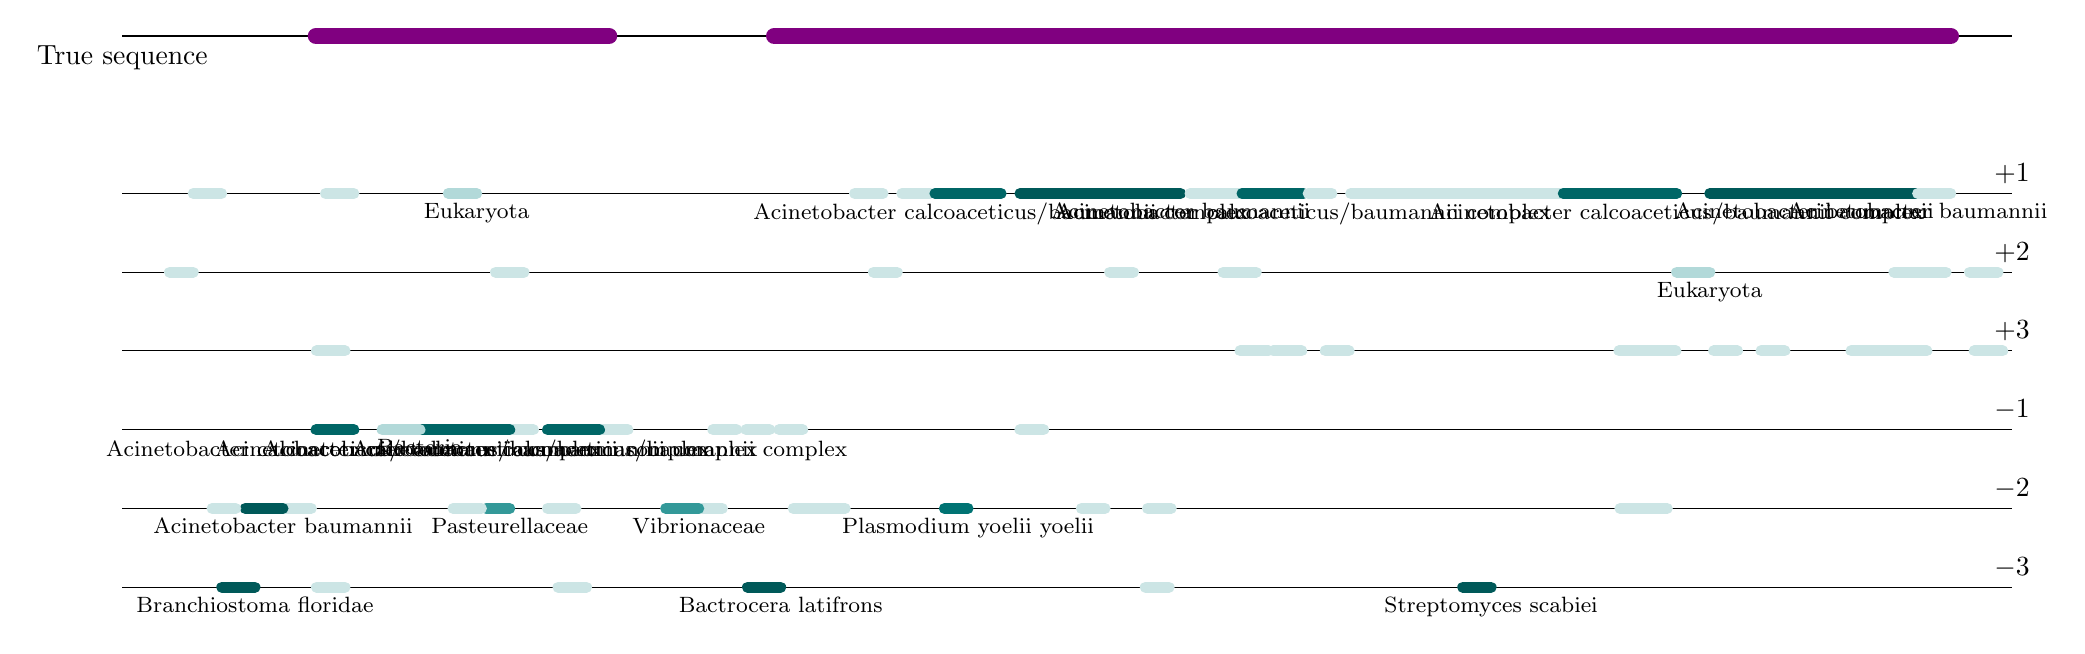
\begin{tikzpicture}
[protein/.style={violet, line width = 6pt, line cap = round},
root/.style={teal!20, line width = 4pt, line cap = round},
genus/.style={teal, line width = 4pt, line cap = round},
subspecies/.style={teal!90!black, line width = 4pt, line cap = round},
species/.style={teal!70!black, line width = 4pt, line cap = round},
species group/.style={teal!80!black, line width = 4pt, line cap = round},
family/.style={teal!80, line width = 4pt, line cap = round},
order/.style={teal!70, line width = 4pt, line cap = round},
class/.style={teal!60, line width = 4pt, line cap = round},
phylum/.style={teal!50, line width = 4pt, line cap = round},
kingdom/.style={teal!40, line width = 4pt, line cap = round},
superkingdom/.style={teal!30, line width = 4pt, line cap = round}]
\draw node[anchor=north] {True sequence} (0,0) -- (24,0) ;
\draw (0,-2) -- (24,-2) node[anchor=south] {$+1$};
\draw (0,-3) -- (24,-3) node[anchor=south] {$+2$};
\draw (0,-4) -- (24,-4) node[anchor=south] {$+3$};
\draw (0,-5) -- (24,-5) node[anchor=south] {$-1$};
\draw (0,-6) -- (24,-6) node[anchor=south] {$-2$};
\draw (0,-7) -- (24,-7) node[anchor=south] {$-3$};
\draw[protein] (8.28,0) -- (23.22,0);
\draw[root] (0.8999999999999999,-2) -- (1.2599999999999998,-2);
\draw[root] (2.58,-2) -- (2.94,-2);
\draw[superkingdom] (4.14,-2) -- (4.5,-2);
\node [below,font=\footnotesize] at (4.5,-2) {Eukaryota};
\draw[root] (9.299999999999999,-2) -- (9.659999999999998,-2);
\draw[root] (9.9,-2) -- (10.26,-2);
\draw[species group] (10.32,-2) -- (11.16,-2);
\node [below,font=\footnotesize] at (11.16,-2) {Acinetobacter calcoaceticus/baumannii complex};
\draw[species] (11.4,-2) -- (13.440000000000001,-2);
\node [below,font=\footnotesize] at (13.440000000000001,-2) {Acinetobacter baumannii};
\draw[root] (13.559999999999999,-2) -- (14.219999999999999,-2);
\draw[species group] (14.219999999999999,-2) -- (14.999999999999998,-2);
\node [below,font=\footnotesize] at (14.999999999999998,-2) {Acinetobacter calcoaceticus/baumannii complex};
\draw[root] (15.059999999999999,-2) -- (15.36,-2);
\draw[root] (15.6,-2) -- (17.34,-2);
\draw[root] (17.34,-2) -- (17.64,-2);
\draw[root] (17.64,-2) -- (18.3,-2);
\draw[species group] (18.3,-2) -- (19.740000000000002,-2);
\node [below,font=\footnotesize] at (19.740000000000002,-2) {Acinetobacter calcoaceticus/baumannii complex};
\draw[species] (20.16,-2) -- (21.36,-2);
\node [below,font=\footnotesize] at (21.36,-2) {Acinetobacter baumannii};
\draw[species] (21.36,-2) -- (22.8,-2);
\node [below,font=\footnotesize] at (22.8,-2) {Acinetobacter baumannii};
\draw[root] (22.8,-2) -- (23.220000000000002,-2);
\draw[root] (0.6,-3) -- (0.8999999999999999,-3);
\draw[root] (4.74,-3) -- (5.1000000000000005,-3);
\draw[root] (9.54,-3) -- (9.84,-3);
\draw[root] (12.54,-3) -- (12.84,-3);
\draw[root] (13.979999999999999,-3) -- (14.399999999999999,-3);
\draw[superkingdom] (19.74,-3) -- (20.16,-3);
\node [below,font=\footnotesize] at (20.16,-3) {Eukaryota};
\draw[root] (22.5,-3) -- (22.86,-3);
\draw[root] (22.86,-3) -- (23.16,-3);
\draw[root] (23.46,-3) -- (23.82,-3);
\draw[root] (2.4661654135338344,-4) -- (2.827067669172932,-4);
\draw[root] (14.19548872180451,-4) -- (14.556390977443609,-4);
\draw[root] (14.616541353383457,-4) -- (14.977443609022554,-4);
\draw[root] (15.278195488721803,-4) -- (15.578947368421051,-4);
\draw[root] (19.00751879699248,-4) -- (19.308270676691727,-4);
\draw[root] (19.308270676691727,-4) -- (19.729323308270676,-4);
\draw[root] (20.210526315789473,-4) -- (20.51127819548872,-4);
\draw[root] (20.81203007518797,-4) -- (21.112781954887218,-4);
\draw[root] (21.954887218045112,-4) -- (22.31578947368421,-4);
\draw[root] (22.31578947368421,-4) -- (22.616541353383457,-4);
\draw[root] (22.616541353383457,-4) -- (22.917293233082706,-4);
\draw[root] (23.518796992481203,-4) -- (23.8796992481203,-4);
\draw[protein] (2.46,0) -- (6.18,0);
\draw[root] (11.4,-5) -- (11.700000000000001,-5);
\draw[root] (8.34,-5) -- (8.64,-5);
\draw[root] (7.920000000000001,-5) -- (8.22,-5);
\draw[root] (7.500000000000001,-5) -- (7.800000000000001,-5);
\draw[root] (6.060000000000001,-5) -- (6.420000000000002,-5);
\draw[species group] (5.400000000000002,-5) -- (6.060000000000002,-5);
\node [below,font=\footnotesize] at (6.060000000000002,-5) {Acinetobacter calcoaceticus/baumannii complex};
\draw[root] (4.920000000000003,-5) -- (5.220000000000002,-5);
\draw[species group] (4.320000000000002,-5) -- (4.920000000000002,-5);
\node [below,font=\footnotesize] at (4.920000000000002,-5) {Acinetobacter calcoaceticus/baumannii complex};
\draw[species group] (3.7800000000000002,-5) -- (4.32,-5);
\node [below,font=\footnotesize] at (4.32,-5) {Acinetobacter calcoaceticus/baumannii complex};
\draw[superkingdom] (3.300000000000001,-5) -- (3.780000000000001,-5);
\node [below,font=\footnotesize] at (3.780000000000001,-5) {Bacteria};
\draw[species group] (2.4600000000000013,-5) -- (2.9400000000000013,-5);
\node [below,font=\footnotesize] at (2.9400000000000013,-5) {Acinetobacter calcoaceticus/baumannii complex};
\draw[root] (19.32,-6) -- (19.62,-6);
\draw[root] (19.02,-6) -- (19.32,-6);
\draw[root] (13.02,-6) -- (13.32,-6);
\draw[root] (12.18,-6) -- (12.48,-6);
\draw[subspecies] (10.44,-6) -- (10.74,-6);
\node [below,font=\footnotesize] at (10.74,-6) {Plasmodium yoelii yoelii};
\draw[root] (8.879999999999999,-6) -- (9.18,-6);
\draw[root] (8.520000000000001,-6) -- (8.88,-6);
\draw[root] (7.320000000000001,-6) -- (7.620000000000001,-6);
\draw[family] (6.9,-6) -- (7.32,-6);
\node [below,font=\footnotesize] at (7.32,-6) {Vibrionaceae};
\draw[root] (5.400000000000001,-6) -- (5.760000000000002,-6);
\draw[family] (4.620000000000002,-6) -- (4.920000000000002,-6);
\node [below,font=\footnotesize] at (4.920000000000002,-6) {Pasteurellaceae};
\draw[root] (4.200000000000002,-6) -- (4.560000000000002,-6);
\draw[root] (2.0400000000000023,-6) -- (2.400000000000002,-6);
\draw[species] (1.5599999999999992,-6) -- (2.039999999999999,-6);
\node [below,font=\footnotesize] at (2.039999999999999,-6) {Acinetobacter baumannii};
\draw[root] (1.1400000000000012,-6) -- (1.4400000000000013,-6);
\draw[species] (17.022556390977446,-7) -- (17.383458646616543,-7);
\node [below,font=\footnotesize] at (17.383458646616543,-7) {Streptomyces scabiei};
\draw[root] (12.992481203007518,-7) -- (13.293233082706767,-7);
\draw[species] (7.939849624060152,-7) -- (8.360902255639099,-7);
\node [below,font=\footnotesize] at (8.360902255639099,-7) {Bactrocera latifrons};
\draw[root] (5.533834586466166,-7) -- (5.894736842105264,-7);
\draw[root] (2.466165413533836,-7) -- (2.8270676691729335,-7);
\draw[species] (1.2631578947368438,-7) -- (1.6842105263157912,-7);
\node [below,font=\footnotesize] at (1.6842105263157912,-7) {Branchiostoma floridae};
\end{tikzpicture}

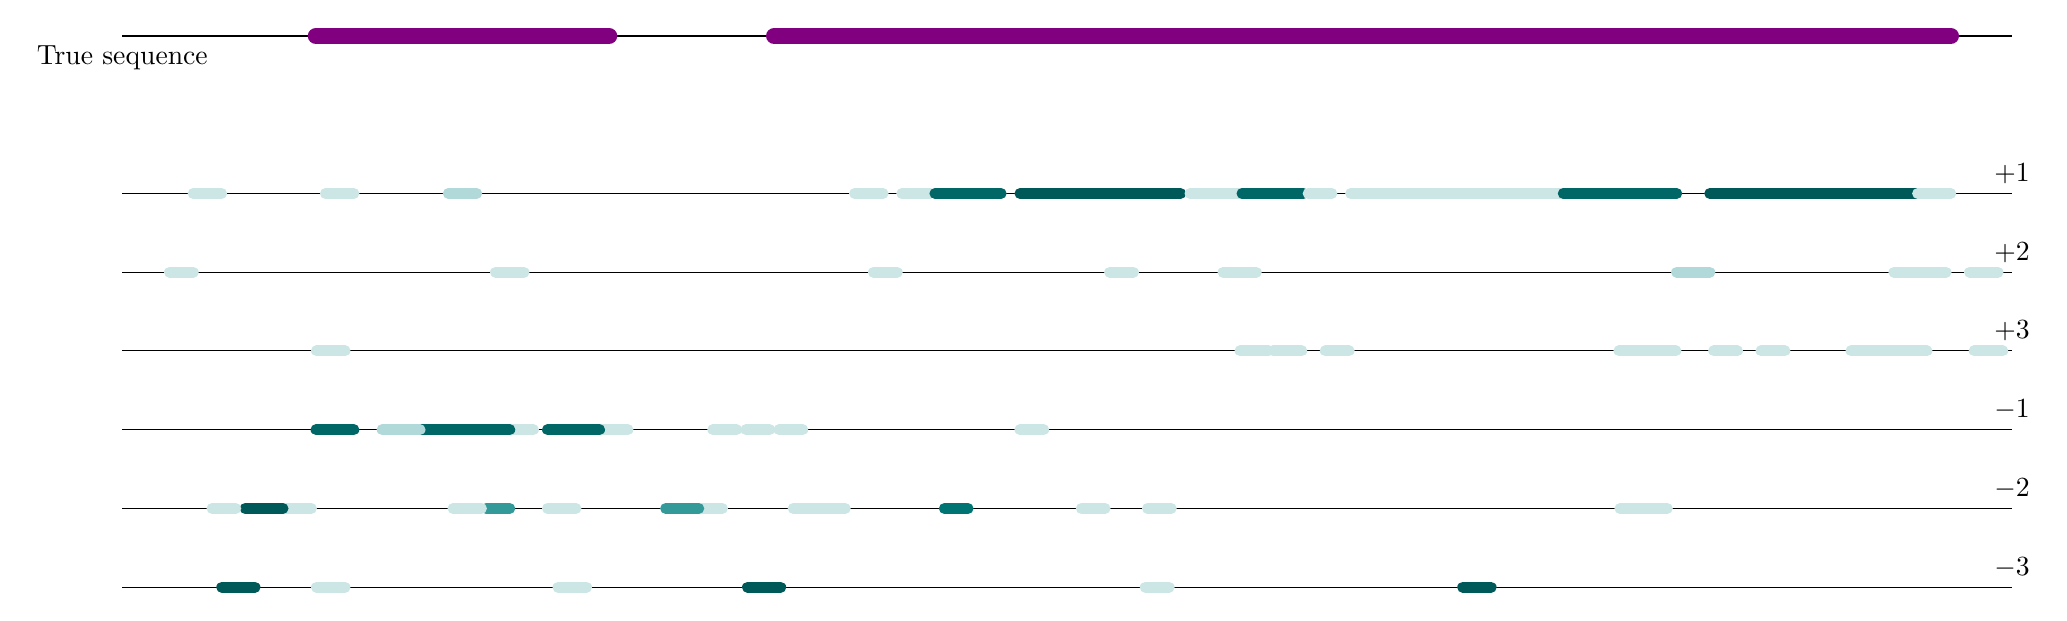
\begin{tikzpicture}
[protein/.style={violet, line width = 6pt, line cap = round},
root/.style={teal!20, line width = 4pt, line cap = round},
genus/.style={teal, line width = 4pt, line cap = round},
subspecies/.style={teal!90!black, line width = 4pt, line cap = round},
species/.style={teal!70!black, line width = 4pt, line cap = round},
species group/.style={teal!80!black, line width = 4pt, line cap = round},
family/.style={teal!80, line width = 4pt, line cap = round},
order/.style={teal!70, line width = 4pt, line cap = round},
class/.style={teal!60, line width = 4pt, line cap = round},
phylum/.style={teal!50, line width = 4pt, line cap = round},
kingdom/.style={teal!40, line width = 4pt, line cap = round},
superkingdom/.style={teal!30, line width = 4pt, line cap = round}]
\draw node[anchor=north] {True sequence} (0,0) -- (24,0) ;
\draw (0,-2) -- (24,-2) node[anchor=south] {$+1$};
\draw (0,-3) -- (24,-3) node[anchor=south] {$+2$};
\draw (0,-4) -- (24,-4) node[anchor=south] {$+3$};
\draw (0,-5) -- (24,-5) node[anchor=south] {$-1$};
\draw (0,-6) -- (24,-6) node[anchor=south] {$-2$};
\draw (0,-7) -- (24,-7) node[anchor=south] {$-3$};
\draw[protein] (8.28,0) -- (23.22,0);
\draw[root] (0.8999999999999999,-2) -- (1.2599999999999998,-2);
\draw[root] (2.58,-2) -- (2.94,-2);
\draw[superkingdom] (4.14,-2) -- (4.5,-2);
\draw[root] (9.299999999999999,-2) -- (9.659999999999998,-2);
\draw[root] (9.9,-2) -- (10.26,-2);
\draw[species group] (10.32,-2) -- (11.16,-2);
\draw[species] (11.4,-2) -- (13.440000000000001,-2);
\draw[root] (13.559999999999999,-2) -- (14.219999999999999,-2);
\draw[species group] (14.219999999999999,-2) -- (14.999999999999998,-2);
\draw[root] (15.059999999999999,-2) -- (15.36,-2);
\draw[root] (15.6,-2) -- (17.34,-2);
\draw[root] (17.34,-2) -- (17.64,-2);
\draw[root] (17.64,-2) -- (18.3,-2);
\draw[species group] (18.3,-2) -- (19.740000000000002,-2);
\draw[species] (20.16,-2) -- (21.36,-2);
\draw[species] (21.36,-2) -- (22.8,-2);
\draw[root] (22.8,-2) -- (23.220000000000002,-2);
\draw[root] (0.6,-3) -- (0.8999999999999999,-3);
\draw[root] (4.74,-3) -- (5.1000000000000005,-3);
\draw[root] (9.54,-3) -- (9.84,-3);
\draw[root] (12.54,-3) -- (12.84,-3);
\draw[root] (13.979999999999999,-3) -- (14.399999999999999,-3);
\draw[superkingdom] (19.74,-3) -- (20.16,-3);
\draw[root] (22.5,-3) -- (22.86,-3);
\draw[root] (22.86,-3) -- (23.16,-3);
\draw[root] (23.46,-3) -- (23.82,-3);
\draw[root] (2.4661654135338344,-4) -- (2.827067669172932,-4);
\draw[root] (14.19548872180451,-4) -- (14.556390977443609,-4);
\draw[root] (14.616541353383457,-4) -- (14.977443609022554,-4);
\draw[root] (15.278195488721803,-4) -- (15.578947368421051,-4);
\draw[root] (19.00751879699248,-4) -- (19.308270676691727,-4);
\draw[root] (19.308270676691727,-4) -- (19.729323308270676,-4);
\draw[root] (20.210526315789473,-4) -- (20.51127819548872,-4);
\draw[root] (20.81203007518797,-4) -- (21.112781954887218,-4);
\draw[root] (21.954887218045112,-4) -- (22.31578947368421,-4);
\draw[root] (22.31578947368421,-4) -- (22.616541353383457,-4);
\draw[root] (22.616541353383457,-4) -- (22.917293233082706,-4);
\draw[root] (23.518796992481203,-4) -- (23.8796992481203,-4);
\draw[protein] (2.46,0) -- (6.18,0);
\draw[root] (11.4,-5) -- (11.700000000000001,-5);
\draw[root] (8.34,-5) -- (8.64,-5);
\draw[root] (7.920000000000001,-5) -- (8.22,-5);
\draw[root] (7.500000000000001,-5) -- (7.800000000000001,-5);
\draw[root] (6.060000000000001,-5) -- (6.420000000000002,-5);
\draw[species group] (5.400000000000002,-5) -- (6.060000000000002,-5);
\draw[root] (4.920000000000003,-5) -- (5.220000000000002,-5);
\draw[species group] (4.320000000000002,-5) -- (4.920000000000002,-5);
\draw[species group] (3.7800000000000002,-5) -- (4.32,-5);
\draw[superkingdom] (3.300000000000001,-5) -- (3.780000000000001,-5);
\draw[species group] (2.4600000000000013,-5) -- (2.9400000000000013,-5);
\draw[root] (19.32,-6) -- (19.62,-6);
\draw[root] (19.02,-6) -- (19.32,-6);
\draw[root] (13.02,-6) -- (13.32,-6);
\draw[root] (12.18,-6) -- (12.48,-6);
\draw[subspecies] (10.44,-6) -- (10.74,-6);
\draw[root] (8.879999999999999,-6) -- (9.18,-6);
\draw[root] (8.520000000000001,-6) -- (8.88,-6);
\draw[root] (7.320000000000001,-6) -- (7.620000000000001,-6);
\draw[family] (6.9,-6) -- (7.32,-6);
\draw[root] (5.400000000000001,-6) -- (5.760000000000002,-6);
\draw[family] (4.620000000000002,-6) -- (4.920000000000002,-6);
\draw[root] (4.200000000000002,-6) -- (4.560000000000002,-6);
\draw[root] (2.0400000000000023,-6) -- (2.400000000000002,-6);
\draw[species] (1.5599999999999992,-6) -- (2.039999999999999,-6);
\draw[root] (1.1400000000000012,-6) -- (1.4400000000000013,-6);
\draw[species] (17.022556390977446,-7) -- (17.383458646616543,-7);
\draw[root] (12.992481203007518,-7) -- (13.293233082706767,-7);
\draw[species] (7.939849624060152,-7) -- (8.360902255639099,-7);
\draw[root] (5.533834586466166,-7) -- (5.894736842105264,-7);
\draw[root] (2.466165413533836,-7) -- (2.8270676691729335,-7);
\draw[species] (1.2631578947368438,-7) -- (1.6842105263157912,-7);
\end{tikzpicture}

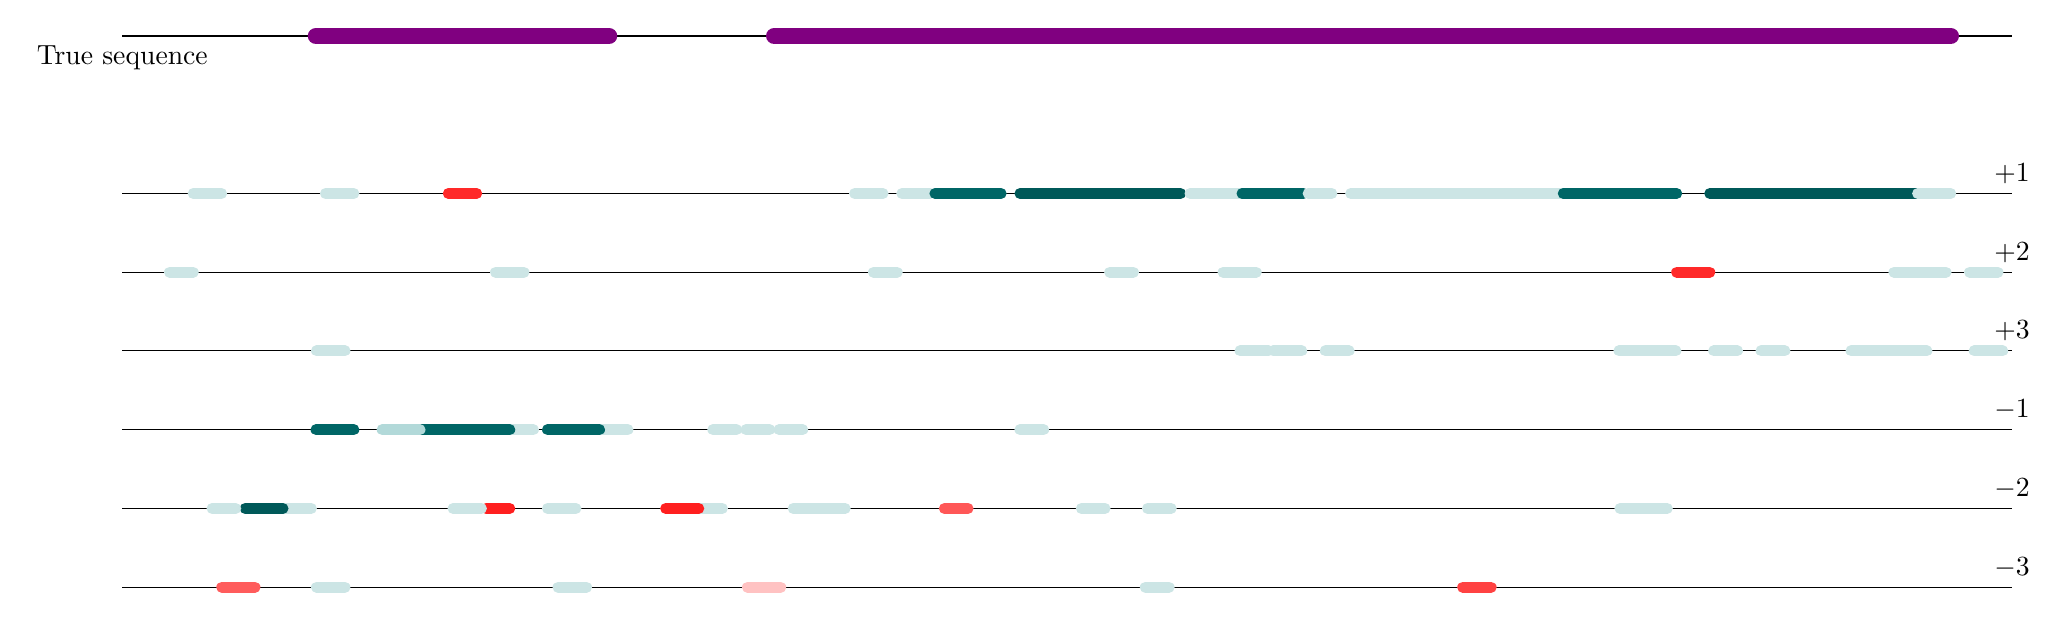
\begin{tikzpicture}
[protein/.style={violet, line width = 6pt, line cap = round},
root/.style={teal!20, line width = 4pt, line cap = round},
genus/.style={teal, line width = 4pt, line cap = round},
subspecies/.style={teal!90!black, line width = 4pt, line cap = round},
species/.style={teal!70!black, line width = 4pt, line cap = round},
species group/.style={teal!80!black, line width = 4pt, line cap = round},
family/.style={teal!80, line width = 4pt, line cap = round},
order/.style={teal!70, line width = 4pt, line cap = round},
class/.style={teal!60, line width = 4pt, line cap = round},
phylum/.style={teal!50, line width = 4pt, line cap = round},
kingdom/.style={teal!40, line width = 4pt, line cap = round},
superkingdom/.style={teal!30, line width = 4pt, line cap = round}]
\draw node[anchor=north] {True sequence} (0,0) -- (24,0) ;
\draw (0,-2) -- (24,-2) node[anchor=south] {$+1$};
\draw (0,-3) -- (24,-3) node[anchor=south] {$+2$};
\draw (0,-4) -- (24,-4) node[anchor=south] {$+3$};
\draw (0,-5) -- (24,-5) node[anchor=south] {$-1$};
\draw (0,-6) -- (24,-6) node[anchor=south] {$-2$};
\draw (0,-7) -- (24,-7) node[anchor=south] {$-3$};
\draw[protein] (8.28,0) -- (23.22,0);
\draw[root] (0.8999999999999999,-2) -- (1.2599999999999998,-2);
\draw[root] (2.58,-2) -- (2.94,-2);
\draw[red!84, line width = 4pt, line cap = round] (4.14,-2) -- (4.5,-2);
\draw[root] (9.299999999999999,-2) -- (9.659999999999998,-2);
\draw[root] (9.9,-2) -- (10.26,-2);
\draw[species group] (10.32,-2) -- (11.16,-2);
\draw[species] (11.4,-2) -- (13.440000000000001,-2);
\draw[root] (13.559999999999999,-2) -- (14.219999999999999,-2);
\draw[species group] (14.219999999999999,-2) -- (14.999999999999998,-2);
\draw[root] (15.059999999999999,-2) -- (15.36,-2);
\draw[root] (15.6,-2) -- (17.34,-2);
\draw[root] (17.34,-2) -- (17.64,-2);
\draw[root] (17.64,-2) -- (18.3,-2);
\draw[species group] (18.3,-2) -- (19.740000000000002,-2);
\draw[species] (20.16,-2) -- (21.36,-2);
\draw[species] (21.36,-2) -- (22.8,-2);
\draw[root] (22.8,-2) -- (23.220000000000002,-2);
\draw[root] (0.6,-3) -- (0.8999999999999999,-3);
\draw[root] (4.74,-3) -- (5.1000000000000005,-3);
\draw[root] (9.54,-3) -- (9.84,-3);
\draw[root] (12.54,-3) -- (12.84,-3);
\draw[root] (13.979999999999999,-3) -- (14.399999999999999,-3);
\draw[red!84, line width = 4pt, line cap = round] (19.74,-3) -- (20.16,-3);
\draw[root] (22.5,-3) -- (22.86,-3);
\draw[root] (22.86,-3) -- (23.16,-3);
\draw[root] (23.46,-3) -- (23.82,-3);
\draw[root] (2.4661654135338344,-4) -- (2.827067669172932,-4);
\draw[root] (14.19548872180451,-4) -- (14.556390977443609,-4);
\draw[root] (14.616541353383457,-4) -- (14.977443609022554,-4);
\draw[root] (15.278195488721803,-4) -- (15.578947368421051,-4);
\draw[root] (19.00751879699248,-4) -- (19.308270676691727,-4);
\draw[root] (19.308270676691727,-4) -- (19.729323308270676,-4);
\draw[root] (20.210526315789473,-4) -- (20.51127819548872,-4);
\draw[root] (20.81203007518797,-4) -- (21.112781954887218,-4);
\draw[root] (21.954887218045112,-4) -- (22.31578947368421,-4);
\draw[root] (22.31578947368421,-4) -- (22.616541353383457,-4);
\draw[root] (22.616541353383457,-4) -- (22.917293233082706,-4);
\draw[root] (23.518796992481203,-4) -- (23.8796992481203,-4);
\draw[protein] (2.46,0) -- (6.18,0);
\draw[root] (11.4,-5) -- (11.700000000000001,-5);
\draw[root] (8.34,-5) -- (8.64,-5);
\draw[root] (7.920000000000001,-5) -- (8.22,-5);
\draw[root] (7.500000000000001,-5) -- (7.800000000000001,-5);
\draw[root] (6.060000000000001,-5) -- (6.420000000000002,-5);
\draw[species group] (5.400000000000002,-5) -- (6.060000000000002,-5);
\draw[root] (4.920000000000003,-5) -- (5.220000000000002,-5);
\draw[species group] (4.320000000000002,-5) -- (4.920000000000002,-5);
\draw[species group] (3.7800000000000002,-5) -- (4.32,-5);
\draw[superkingdom] (3.300000000000001,-5) -- (3.780000000000001,-5);
\draw[species group] (2.4600000000000013,-5) -- (2.9400000000000013,-5);
\draw[root] (19.32,-6) -- (19.62,-6);
\draw[root] (19.02,-6) -- (19.32,-6);
\draw[root] (13.02,-6) -- (13.32,-6);
\draw[root] (12.18,-6) -- (12.48,-6);
\draw[red!66, line width = 4pt, line cap = round] (10.44,-6) -- (10.74,-6);
\draw[root] (8.879999999999999,-6) -- (9.18,-6);
\draw[root] (8.520000000000001,-6) -- (8.88,-6);
\draw[root] (7.320000000000001,-6) -- (7.620000000000001,-6);
\draw[red!88, line width = 4pt, line cap = round] (6.9,-6) -- (7.32,-6);
\draw[root] (5.400000000000001,-6) -- (5.760000000000002,-6);
\draw[red!88, line width = 4pt, line cap = round] (4.620000000000002,-6) -- (4.920000000000002,-6);
\draw[root] (4.200000000000002,-6) -- (4.560000000000002,-6);
\draw[root] (2.0400000000000023,-6) -- (2.400000000000002,-6);
\draw[species] (1.5599999999999992,-6) -- (2.039999999999999,-6);
\draw[root] (1.1400000000000012,-6) -- (1.4400000000000013,-6);
\draw[red!74, line width = 4pt, line cap = round] (17.022556390977446,-7) -- (17.383458646616543,-7);
\draw[root] (12.992481203007518,-7) -- (13.293233082706767,-7);
\draw[red!24, line width = 4pt, line cap = round] (7.939849624060152,-7) -- (8.360902255639099,-7);
\draw[root] (5.533834586466166,-7) -- (5.894736842105264,-7);
\draw[root] (2.466165413533836,-7) -- (2.8270676691729335,-7);
\draw[red!64, line width = 4pt, line cap = round] (1.2631578947368438,-7) -- (1.6842105263157912,-7);
\end{tikzpicture}

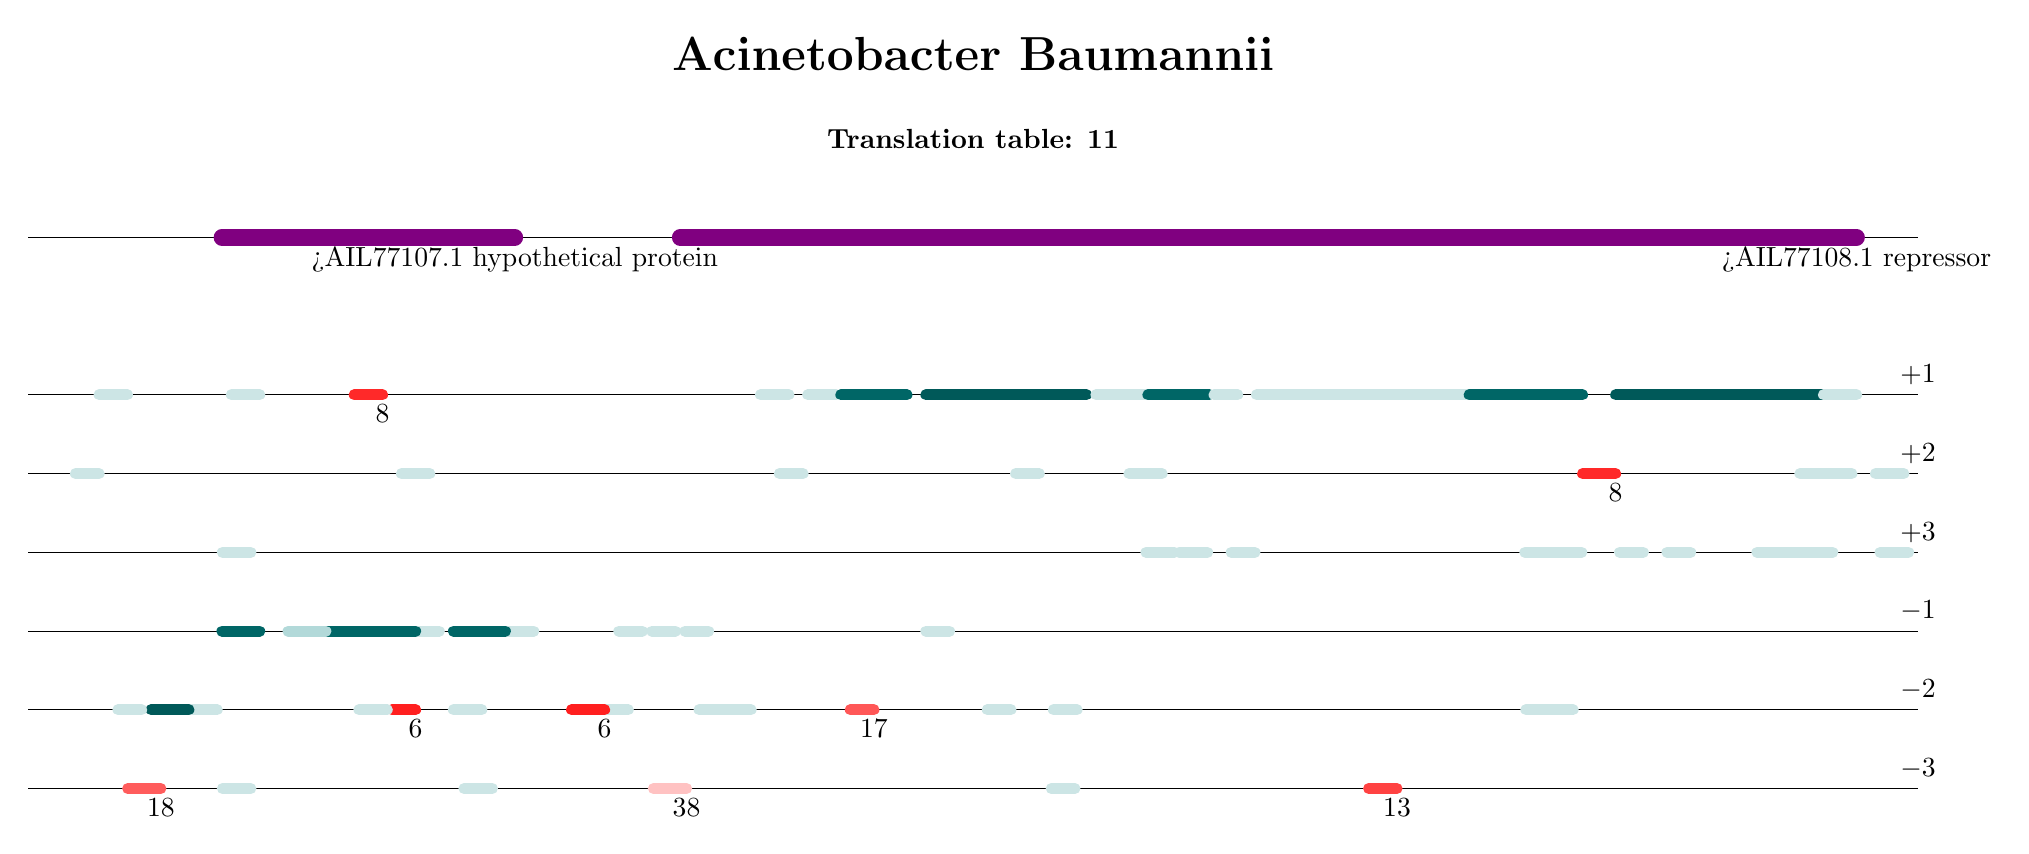
\begin{tikzpicture}
[protein/.style={violet, line width = 6pt, line cap = round},
root/.style={teal!20, line width = 4pt, line cap = round},
genus/.style={teal, line width = 4pt, line cap = round},
subspecies/.style={teal!90!black, line width = 4pt, line cap = round},
species/.style={teal!70!black, line width = 4pt, line cap = round},
species group/.style={teal!80!black, line width = 4pt, line cap = round},
family/.style={teal!80, line width = 4pt, line cap = round},
order/.style={teal!70, line width = 4pt, line cap = round},
class/.style={teal!60, line width = 4pt, line cap = round},
phylum/.style={teal!50, line width = 4pt, line cap = round},
kingdom/.style={teal!40, line width = 4pt, line cap = round},
superkingdom/.style={teal!30, line width = 4pt, line cap = round}]
\node[font=\bfseries\LARGE,align=center,above] at (12,2) {Acinetobacter Baumannii} ;
\node[font=\bfseries,align=center,above] at (12,1) {Translation table: 11} ;
\draw (0,0) -- (24,0) ;
\draw (0,-2) -- (24,-2) node[anchor=south] {$+1$};
\draw (0,-3) -- (24,-3) node[anchor=south] {$+2$};
\draw (0,-4) -- (24,-4) node[anchor=south] {$+3$};
\draw (0,-5) -- (24,-5) node[anchor=south] {$-1$};
\draw (0,-6) -- (24,-6) node[anchor=south] {$-2$};
\draw (0,-7) -- (24,-7) node[anchor=south] {$-3$};
\draw[protein] (8.28,0) -- (23.22,0);
\node[below] at (23.22,0)  {>AIL77108.1 repressor};
\draw[root] (0.8999999999999999,-2) -- (1.2599999999999998,-2);
\draw[root] (2.58,-2) -- (2.94,-2);
\draw[red!84, line width = 4pt, line cap = round] (4.14,-2) -- (4.5,-2);
\node[below] at (4.5,-2) {8};
\draw[root] (9.299999999999999,-2) -- (9.659999999999998,-2);
\draw[root] (9.9,-2) -- (10.26,-2);
\draw[species group] (10.32,-2) -- (11.16,-2);
\draw[species] (11.4,-2) -- (13.440000000000001,-2);
\draw[root] (13.559999999999999,-2) -- (14.219999999999999,-2);
\draw[species group] (14.219999999999999,-2) -- (14.999999999999998,-2);
\draw[root] (15.059999999999999,-2) -- (15.36,-2);
\draw[root] (15.6,-2) -- (17.34,-2);
\draw[root] (17.34,-2) -- (17.64,-2);
\draw[root] (17.64,-2) -- (18.3,-2);
\draw[species group] (18.3,-2) -- (19.740000000000002,-2);
\draw[species] (20.16,-2) -- (21.36,-2);
\draw[species] (21.36,-2) -- (22.8,-2);
\draw[root] (22.8,-2) -- (23.220000000000002,-2);
\draw[root] (0.6,-3) -- (0.8999999999999999,-3);
\draw[root] (4.74,-3) -- (5.1000000000000005,-3);
\draw[root] (9.54,-3) -- (9.84,-3);
\draw[root] (12.54,-3) -- (12.84,-3);
\draw[root] (13.979999999999999,-3) -- (14.399999999999999,-3);
\draw[red!84, line width = 4pt, line cap = round] (19.74,-3) -- (20.16,-3);
\node[below] at (20.16,-3) {8};
\draw[root] (22.5,-3) -- (22.86,-3);
\draw[root] (22.86,-3) -- (23.16,-3);
\draw[root] (23.46,-3) -- (23.82,-3);
\draw[root] (2.4661654135338344,-4) -- (2.827067669172932,-4);
\draw[root] (14.19548872180451,-4) -- (14.556390977443609,-4);
\draw[root] (14.616541353383457,-4) -- (14.977443609022554,-4);
\draw[root] (15.278195488721803,-4) -- (15.578947368421051,-4);
\draw[root] (19.00751879699248,-4) -- (19.308270676691727,-4);
\draw[root] (19.308270676691727,-4) -- (19.729323308270676,-4);
\draw[root] (20.210526315789473,-4) -- (20.51127819548872,-4);
\draw[root] (20.81203007518797,-4) -- (21.112781954887218,-4);
\draw[root] (21.954887218045112,-4) -- (22.31578947368421,-4);
\draw[root] (22.31578947368421,-4) -- (22.616541353383457,-4);
\draw[root] (22.616541353383457,-4) -- (22.917293233082706,-4);
\draw[root] (23.518796992481203,-4) -- (23.8796992481203,-4);
\draw[protein] (2.46,0) -- (6.18,0);
\node[below] at (6.18,0) {>AIL77107.1 hypothetical protein};
\draw[root] (11.4,-5) -- (11.700000000000001,-5);
\draw[root] (8.34,-5) -- (8.64,-5);
\draw[root] (7.920000000000001,-5) -- (8.22,-5);
\draw[root] (7.500000000000001,-5) -- (7.800000000000001,-5);
\draw[root] (6.060000000000001,-5) -- (6.420000000000002,-5);
\draw[species group] (5.400000000000002,-5) -- (6.060000000000002,-5);
\draw[root] (4.920000000000003,-5) -- (5.220000000000002,-5);
\draw[species group] (4.320000000000002,-5) -- (4.920000000000002,-5);
\draw[species group] (3.7800000000000002,-5) -- (4.32,-5);
\draw[superkingdom] (3.300000000000001,-5) -- (3.780000000000001,-5);
\draw[species group] (2.4600000000000013,-5) -- (2.9400000000000013,-5);
\draw[root] (19.32,-6) -- (19.62,-6);
\draw[root] (19.02,-6) -- (19.32,-6);
\draw[root] (13.02,-6) -- (13.32,-6);
\draw[root] (12.18,-6) -- (12.48,-6);
\draw[red!66, line width = 4pt, line cap = round] (10.44,-6) -- (10.74,-6);
\node[below] at (10.74,-6) {17};
\draw[root] (8.879999999999999,-6) -- (9.18,-6);
\draw[root] (8.520000000000001,-6) -- (8.88,-6);
\draw[root] (7.320000000000001,-6) -- (7.620000000000001,-6);
\draw[red!88, line width = 4pt, line cap = round] (6.9,-6) -- (7.32,-6);
\node[below] at (7.32,-6) {6};
\draw[root] (5.400000000000001,-6) -- (5.760000000000002,-6);
\draw[red!88, line width = 4pt, line cap = round] (4.620000000000002,-6) -- (4.920000000000002,-6);
\node[below] at (4.920000000000002,-6) {6};
\draw[root] (4.200000000000002,-6) -- (4.560000000000002,-6);
\draw[root] (2.0400000000000023,-6) -- (2.400000000000002,-6);
\draw[species] (1.5599999999999992,-6) -- (2.039999999999999,-6);
\draw[root] (1.1400000000000012,-6) -- (1.4400000000000013,-6);
\draw[red!74, line width = 4pt, line cap = round] (17.022556390977446,-7) -- (17.383458646616543,-7);
\node[below] at (17.383458646616543,-7) {13};
\draw[root] (12.992481203007518,-7) -- (13.293233082706767,-7);
\draw[red!24, line width = 4pt, line cap = round] (7.939849624060152,-7) -- (8.360902255639099,-7);
\node[below] at (8.360902255639099,-7) {38};
\draw[root] (5.533834586466166,-7) -- (5.894736842105264,-7);
\draw[root] (2.466165413533836,-7) -- (2.8270676691729335,-7);
\draw[red!64, line width = 4pt, line cap = round] (1.2631578947368438,-7) -- (1.6842105263157912,-7);
\node[below] at (1.6842105263157912,-7) {18};
\end{tikzpicture}


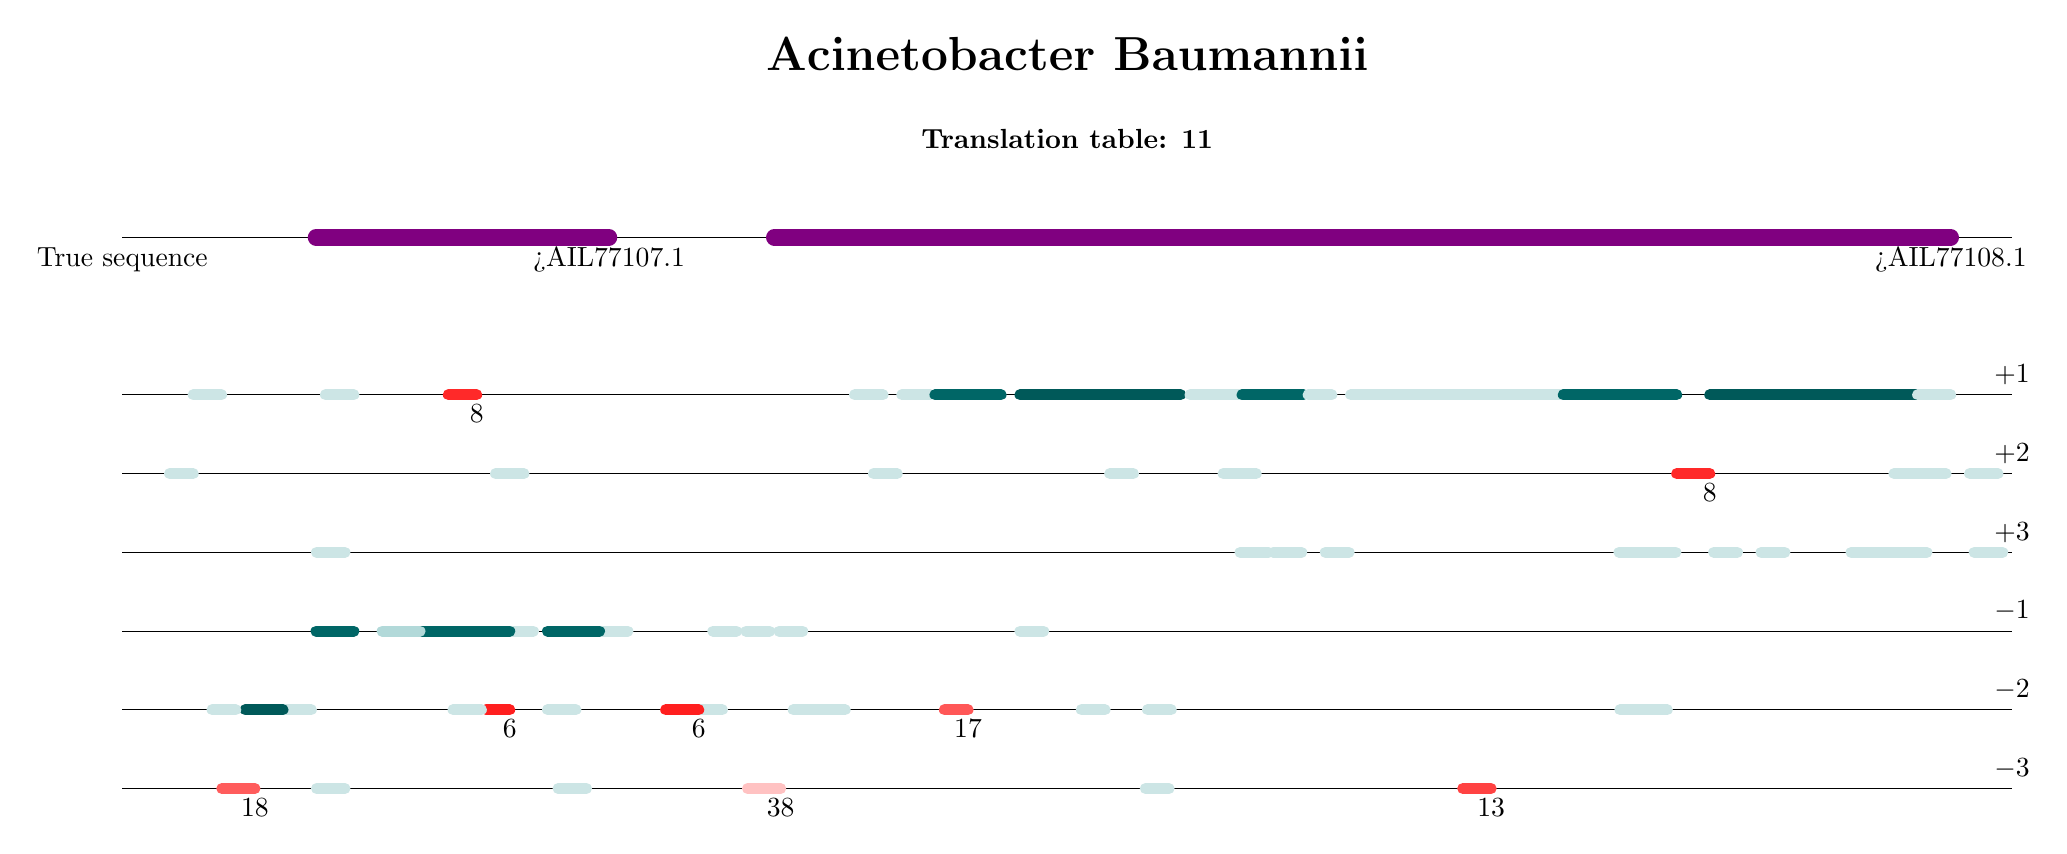
\begin{tikzpicture}
[protein/.style={violet, line width = 6pt, line cap = round},
root/.style={teal!20, line width = 4pt, line cap = round},
genus/.style={teal, line width = 4pt, line cap = round},
subspecies/.style={teal!90!black, line width = 4pt, line cap = round},
species/.style={teal!70!black, line width = 4pt, line cap = round},
species group/.style={teal!80!black, line width = 4pt, line cap = round},
family/.style={teal!80, line width = 4pt, line cap = round},
order/.style={teal!70, line width = 4pt, line cap = round},
class/.style={teal!60, line width = 4pt, line cap = round},
phylum/.style={teal!50, line width = 4pt, line cap = round},
kingdom/.style={teal!40, line width = 4pt, line cap = round},
superkingdom/.style={teal!30, line width = 4pt, line cap = round}]
\node[font=\bfseries\LARGE,align=center,above] at (12,2) {Acinetobacter Baumannii} ;
\node[font=\bfseries,align=center,above] at (12,1) {Translation table: 11} ;
\draw node[anchor=north] {True sequence} (0,0) -- (24,0) ;
\draw (0,-2) -- (24,-2) node[anchor=south] {$+1$};
\draw (0,-3) -- (24,-3) node[anchor=south] {$+2$};
\draw (0,-4) -- (24,-4) node[anchor=south] {$+3$};
\draw (0,-5) -- (24,-5) node[anchor=south] {$-1$};
\draw (0,-6) -- (24,-6) node[anchor=south] {$-2$};
\draw (0,-7) -- (24,-7) node[anchor=south] {$-3$};
\draw[protein] (8.28,0) -- (23.22,0);
\node[below] at (23.22,0)  {>AIL77108.1};
\draw[root] (0.8999999999999999,-2) -- (1.2599999999999998,-2);
\draw[root] (2.58,-2) -- (2.94,-2);
\draw[red!84, line width = 4pt, line cap = round] (4.14,-2) -- (4.5,-2);
\node[below] at (4.5,-2) {8};
\draw[root] (9.299999999999999,-2) -- (9.659999999999998,-2);
\draw[root] (9.9,-2) -- (10.26,-2);
\draw[species group] (10.32,-2) -- (11.16,-2);
\draw[species] (11.4,-2) -- (13.440000000000001,-2);
\draw[root] (13.559999999999999,-2) -- (14.219999999999999,-2);
\draw[species group] (14.219999999999999,-2) -- (14.999999999999998,-2);
\draw[root] (15.059999999999999,-2) -- (15.36,-2);
\draw[root] (15.6,-2) -- (17.34,-2);
\draw[root] (17.34,-2) -- (17.64,-2);
\draw[root] (17.64,-2) -- (18.3,-2);
\draw[species group] (18.3,-2) -- (19.740000000000002,-2);
\draw[species] (20.16,-2) -- (21.36,-2);
\draw[species] (21.36,-2) -- (22.8,-2);
\draw[root] (22.8,-2) -- (23.220000000000002,-2);
\draw[root] (0.6,-3) -- (0.8999999999999999,-3);
\draw[root] (4.74,-3) -- (5.1000000000000005,-3);
\draw[root] (9.54,-3) -- (9.84,-3);
\draw[root] (12.54,-3) -- (12.84,-3);
\draw[root] (13.979999999999999,-3) -- (14.399999999999999,-3);
\draw[red!84, line width = 4pt, line cap = round] (19.74,-3) -- (20.16,-3);
\node[below] at (20.16,-3) {8};
\draw[root] (22.5,-3) -- (22.86,-3);
\draw[root] (22.86,-3) -- (23.16,-3);
\draw[root] (23.46,-3) -- (23.82,-3);
\draw[root] (2.4661654135338344,-4) -- (2.827067669172932,-4);
\draw[root] (14.19548872180451,-4) -- (14.556390977443609,-4);
\draw[root] (14.616541353383457,-4) -- (14.977443609022554,-4);
\draw[root] (15.278195488721803,-4) -- (15.578947368421051,-4);
\draw[root] (19.00751879699248,-4) -- (19.308270676691727,-4);
\draw[root] (19.308270676691727,-4) -- (19.729323308270676,-4);
\draw[root] (20.210526315789473,-4) -- (20.51127819548872,-4);
\draw[root] (20.81203007518797,-4) -- (21.112781954887218,-4);
\draw[root] (21.954887218045112,-4) -- (22.31578947368421,-4);
\draw[root] (22.31578947368421,-4) -- (22.616541353383457,-4);
\draw[root] (22.616541353383457,-4) -- (22.917293233082706,-4);
\draw[root] (23.518796992481203,-4) -- (23.8796992481203,-4);
\draw[protein] (2.46,0) -- (6.18,0);
\node[below] at (6.18,0)  {>AIL77107.1};
\draw[root] (11.4,-5) -- (11.700000000000001,-5);
\draw[root] (8.34,-5) -- (8.64,-5);
\draw[root] (7.920000000000001,-5) -- (8.22,-5);
\draw[root] (7.500000000000001,-5) -- (7.800000000000001,-5);
\draw[root] (6.060000000000001,-5) -- (6.420000000000002,-5);
\draw[species group] (5.400000000000002,-5) -- (6.060000000000002,-5);
\draw[root] (4.920000000000003,-5) -- (5.220000000000002,-5);
\draw[species group] (4.320000000000002,-5) -- (4.920000000000002,-5);
\draw[species group] (3.7800000000000002,-5) -- (4.32,-5);
\draw[superkingdom] (3.300000000000001,-5) -- (3.780000000000001,-5);
\draw[species group] (2.4600000000000013,-5) -- (2.9400000000000013,-5);
\draw[root] (19.32,-6) -- (19.62,-6);
\draw[root] (19.02,-6) -- (19.32,-6);
\draw[root] (13.02,-6) -- (13.32,-6);
\draw[root] (12.18,-6) -- (12.48,-6);
\draw[red!66, line width = 4pt, line cap = round] (10.44,-6) -- (10.74,-6);
\node[below] at (10.74,-6) {17};
\draw[root] (8.879999999999999,-6) -- (9.18,-6);
\draw[root] (8.520000000000001,-6) -- (8.88,-6);
\draw[root] (7.320000000000001,-6) -- (7.620000000000001,-6);
\draw[red!88, line width = 4pt, line cap = round] (6.9,-6) -- (7.32,-6);
\node[below] at (7.32,-6) {6};
\draw[root] (5.400000000000001,-6) -- (5.760000000000002,-6);
\draw[red!88, line width = 4pt, line cap = round] (4.620000000000002,-6) -- (4.920000000000002,-6);
\node[below] at (4.920000000000002,-6) {6};
\draw[root] (4.200000000000002,-6) -- (4.560000000000002,-6);
\draw[root] (2.0400000000000023,-6) -- (2.400000000000002,-6);
\draw[species] (1.5599999999999992,-6) -- (2.039999999999999,-6);
\draw[root] (1.1400000000000012,-6) -- (1.4400000000000013,-6);
\draw[red!74, line width = 4pt, line cap = round] (17.022556390977446,-7) -- (17.383458646616543,-7);
\node[below] at (17.383458646616543,-7) {13};
\draw[root] (12.992481203007518,-7) -- (13.293233082706767,-7);
\draw[red!24, line width = 4pt, line cap = round] (7.939849624060152,-7) -- (8.360902255639099,-7);
\node[below] at (8.360902255639099,-7) {38};
\draw[root] (5.533834586466166,-7) -- (5.894736842105264,-7);
\draw[root] (2.466165413533836,-7) -- (2.8270676691729335,-7);
\draw[red!64, line width = 4pt, line cap = round] (1.2631578947368438,-7) -- (1.6842105263157912,-7);
\node[below] at (1.6842105263157912,-7) {18};
\end{tikzpicture}
\end{document}
